\documentclass{beamer}

% % % % % % % % % % % % % % % % % % % % 
% Preblem
%
\usetheme{metropolis}
\usepackage[backend=bibtex,style=authoryear]{biblatex}
\addbibresource{references.bib}

% add commar between name and year \ Default (Name Year), Renew (Name, Year)
\renewcommand*{\nameyeardelim}{\addcomma\addspace}

% - - - - - - - - - - - - - - - - - - - -
% NEED BY \makethesiscover
% - - - - - - - - - - - - - - - - - - - -
% Common
\newcommand{\studentEmailaddress}{sitdhibong.l@student.chula.ac.th}
% English letters
\newcommand{\ThesisNameEN}{Test Case Generation from a Java Static Call Graph}
\newcommand{\authorNameEN}{Sitdhibong Laokok}
\newcommand{\prefixEN}{Mr.}
\newcommand{\studentnameEn}{{\prefixEN}~{\authorNameEN}}
\newcommand{\curriculumnEn}{Master of Science}
\newcommand{\majorEn}{Software Engineering}
\newcommand{\departmentEn}{Computer Engineering}
\newcommand{\facultyEn}{Faculty of Engineering}
\newcommand{\universityEn}{Chulalongkorn University}
\newcommand{\disclaiminationEn}{Copyright Year 2016}
\newcommand{\advisorEn}{Assoc. Prof. Taratip Suwannasart, Ph.D.}
\newcommand{\engkeywords}{Test case generation, Java language, Static call graph}
\newcommand{\academicYearEn}{2016}


\usepackage[font=scriptsize]{caption}
\usepackage{mwe}

\definecolor{brewcolorRed}{RGB}{150,4,12}

\setbeamercolor{frametitle}{fg=white,bg=brewcolorRed}

\metroset{%
    progressbar=head
}

\useinnertheme{rectangles}

\defbeamertemplate*{footline}{}%
{
    \leavevmode%
    \hbox{%
        \begin{beamercolorbox}[wd=.3\paperwidth,ht=2ex,dp=2ex,center]{section in footer}%
            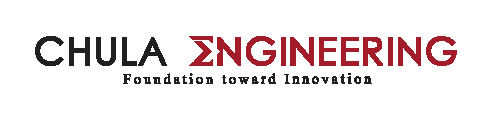
\includegraphics[width=0.25\paperwidth]{figure/chula-engineering}
        \end{beamercolorbox}

        \begin{beamercolorbox}[wd=.5\paperwidth,ht=2ex,dp=2ex,center]{subsection in footer}%
            \insertsubsection
            \vspace{0.2cm}
        \end{beamercolorbox}

        \begin{beamercolorbox}[wd=.2\paperwidth,ht=6ex,dp=2ex,right]{pagenumber in footer}%
            \vfill
            \insertframenumber{}\hspace{1cm}
            \vspace{0.2cm}
        \end{beamercolorbox}
    }
}

% % % % % % % % % % % % % % % % % % % % 

% % % % % % % % % % % % % % % % % % % % 
% Title config
%
\title{\ThesisNameEN}
\subtitle{IMECS2017}
\date[2017.03.14]{\today}
\author{\authorNameEN~\small{and~\advisorEn}}
\institute{{\facultyEn}, {\universityEn}}
% % % % % % % % % % % % % % % % % % % % 

\begin{document}

\maketitle

\begin{frame}[t]{Outline}
    \tableofcontents[hideallsubsections]
\end{frame}

% % % % % % % % % % % % % % % % % % % % 
% Introduction
%
\section{Introduction}
\begin{frame}{Software Testing's benefits}
  \begin{itemize}
     \item Indicating the confidencial level of Software Under Test
     \item Indicating the confidencial level of Software Under Test
     \item Verifying conformance to Software Requirements Specification
     \item Discovering errors in source code
  \end{itemize}
\end{frame}

\begin{frame}{Various Platforms}
    \begin{figure}
        
\includegraphics[width=.8\paperwidth]{figure/mobile_bugs}
        \caption{Various platforms for software}
        \label{fig:variousplatform}
    \end{figure}
\end{frame}

\begin{frame}{Languages}
    \begin{figure}
        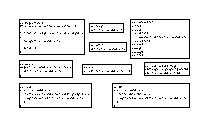
\includegraphics[width=.9\paperwidth]{figure/hello-world-lang}
        \caption{Hello World! in differences languages}
        \label{fig:helloworld}
    \end{figure}
\end{frame}

\begin{frame}{Faults Detection Metric}
    \begin{figure}
        \begin{equation}
            APFD~=~1-~\frac{\sum^{num_f}_{i=1}{TF_i}}{{num}_t \cdot {num}_f} %
                    +~\frac{1}{2 \cdot {num}_t}
            \label{eq:apfd}
        \end{equation}
        \caption{Average Percentage Faults Detected metric \parencite{792604}}
        \label{fig:apfd}
    \end{figure}
\end{frame}

% % % % % % % % % % % % % % % % % % % % 

% % % % % % % % % % % % % % % % % % % % 
% Related works
%
\section{Related works}
\begin{frame}{Automatic Test Case Generation Using Sequence Diagram}
\end{frame}

\begin{frame}{Data flow based Test Case Generation Algorithm for Object Oriented Integration Testing}
\end{frame}
% % % % % % % % % % % % % % % % % % % % 

% % % % % % % % % % % % % % % % % % % % 
% Background
%
\section{Background}
\subsection{Program graph}
\begin{frame}{Program graph}
    \begin{enumerate}
        \item Control Flow Graph
        \item Static Call Graph
    \end{enumerate}
\end{frame}

\begin{frame}{Control Flow Graph}
    \textbf{Control flow graph definition}
    \parencite{Allen:1970:CFA:390013.808479}
\end{frame}

\begin{frame}{Control Flow Graph}
    \begin{figure}
        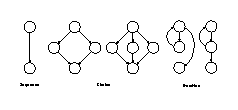
\includegraphics[width=0.7\paperwidth]{figure/Primitive-Operation-Structure}
        \caption{Primitive operation structure \parencite{McCabe1976}}
        \label{fig:primitivestructure}
    \end{figure}
\end{frame}

\begin{frame}{Program graph}
    \begin{enumerate}
        \item<1-> Control Flow Graph
        \item<2-> Static Call Graph
    \end{enumerate}
\end{frame}

\begin{frame}{Static Call Graph}
    \textbf{Static call graph's definition}
\end{frame}

\begin{frame}{Static Call Graph}
    \textbf{Example}
\end{frame}

\begin{frame}{Static Call Graph}
    \begin{figure}
        
\includegraphics[width=0.6\paperwidth]{figure/SCG-A-and-B}
        \caption{Static Call Graph of Class A and Class B}
        \label{fig:staticCallGraphAandB}
    \end{figure}
\end{frame}

% % % % % % % % % % % % % % % % % % % % 

% % % % % % % % % % % % % % % % % % % % 
% Proposed approach
%
\section{Proposed Approach}
\subsection{Overview}
\begin{frame}{Methodology overview}
    \begin{figure}
        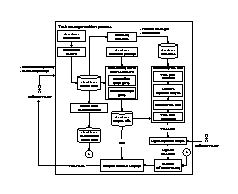
\includegraphics[height=0.65\paperheight]{figure/Methodology.eps}
        \caption{Methodology of Test Case Generation based on Static Data}
        \label{fig:methodologyOverview}
    \end{figure}
\end{frame}

\subsection{Constant collection}
\begin{frame}{Constant collection}
\end{frame}

\subsection{Constructing source code's structure}
\begin{frame}{Constructing source code's structure}
\end{frame}

\subsection{Source code instrumentation}
\begin{frame}{Source code instrumentation}
\end{frame}

\subsection{Generating Test case}
\begin{frame}{Generating Test case}
\end{frame}

\begin{frame}
    \begin{figure}
        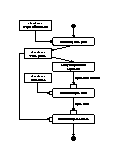
\includegraphics[height=.8\paperheight]{figure/Activities}
        \caption{Test case generation}
        \label{fig:testcasegenearation}
    \end{figure}
\end{frame}

\begin{frame}{Selecting test path}
\end{frame}

\begin{frame}{Selecting test path}
\end{frame}

\begin{frame}{Analizing method signature}
\end{frame}

\begin{frame}{Random input data}
\end{frame}

\begin{frame}{Generating test case}
    \begin{figure}
        \includegraphics<1>[height=.6\paperheight]{figure/Calling-statements-of-Classes}
        \includegraphics<2>[height=.6\paperheight]{figure/Calling-statements-of-Classes-1}
        \includegraphics<3>[height=.6\paperheight]{figure/Calling-statements-of-Classes-2}
        \includegraphics<4>[height=.6\paperheight]{figure/Calling-statements-of-Classes-3}
        \includegraphics<5>[height=.6\paperheight]{figure/Calling-statements-of-Classes-4}
        \includegraphics<6>[height=.6\paperheight]{figure/Calling-statements-of-Classes-5}
        \caption{Calling Statement between Method $m_{11}$, $m_{21}$ and $m_{31}$ of Class $C_1$, $C_2$ and $C_3$ respectively }
        \label{fig:testcasegenearation}
    \end{figure}
\end{frame}

\subsection{Adjust expected output}
\begin{frame}{Adjust expected output}
\end{frame}

\subsection{Execute software testing}
\begin{frame}{Execute software testing}
\end{frame}

\subsection{Compare executed result with graph}
\begin{frame}{Execute software testing}
\end{frame}
% % % % % % % % % % % % % % % % % % % % 

% % % % % % % % % % % % % % % % % % % % 
% Conclusion
%
\section{Conclusion}
\begin{frame}{Conclusion}
    \begin{itemize}
        \item<1->aaaa
        \item<2->bbbb
        \item<3->cccc
    \end{itemize}
\end{frame}
% % % % % % % % % % % % % % % % % % % % 

% % % % % % % % % % % % % % % % % % % % 
% Conclusion
%
\begin{frame}[standout]
    Question \& Answer
\end{frame}
% % % % % % % % % % % % % % % % % % % % 
\end{document}
